% Lecture Template for ME3050 - Dynamic Modeling and Controls - Tennessee Technological University
% Spring 2024 - condensing and streamlining lectures by combining topics into a single PDF under the module name
% this will simplify file and link management as well as make lectures easier to use in class
% - added image/ to clean directory and reduce redundancy, specific to module for now  

% Module Name: - Time Response
% Topic 1 - First Order Time Response
% Topic 2 - Second Order Time Response
% Topic 3 - Response and Root Location
% Topic 4 - Specification of The Step Response

\documentclass[fleqn]{beamer} % for presentation (has nav buttons at bottom)

%\usepackage{/home/tntech.edu/thill/courses/dmc/lectures/dmc_lectures}
%\usepackage{/home/thill/courses/dmc/lectures/dmc_lectures}
\usepackage{/mnt/c/Users/thill/Documents/courses/dmc/lectures/dmc_lectures}

\author{ME3050 - Dynamics Modeling and Controls}

\newcommand{\MNUM}{2\hspace{2mm}} % module number 
\newcommand{\moduletitle}{Time Response}

\newcommand{\sectionItitle}{First Order Time Response}
\newcommand{\sectionIItitle}{Second Order Time Response}
\newcommand{\sectionIIItitle}{Response and Root Location}
\newcommand{\sectionIVtitle}{Specification of The Step Response}

\newcommand{\sectionIsubsectionItitle}{Second Order Free Response}
\newcommand{\sectionIsubsectionIItitle}{Second Order Forced Response}
\newcommand{\sectionIsubsectionIIItitle}{Response and System Stability}
\newcommand{\sectionIsubsectionIVtitle}{Equation Components}

\newcommand{\sectionIIsubsectionItitle}{Damped Natural Frequency and Damping Ratio}
\newcommand{\sectionIIsubsectionIItitle}{The Overdamped Case}
\newcommand{\sectionIIsubsectionIIItitle}{The Critically Damped Case}
\newcommand{\sectionIIsubsectionIVtitle}{The Underdamped Case}

\newcommand{\sectionIIIsubsectionItitle}{The Complex Plane}
\newcommand{\sectionIIIsubsectionIItitle}{Along a Vertical Line}
\newcommand{\sectionIIIsubsectionIIItitle}{Along a Horizontal Line}
\newcommand{\sectionIIIsubsectionIVtitle}{Along a Diagonal Line}

\newcommand{\sectionIVsubsectionItitle}{The Unit Step Response}
\newcommand{\sectionIVsubsectionIItitle}{Rise, Peak, and Settling Time}
\newcommand{\sectionIVsubsectionIIItitle}{Maximum Overshoot and The Damping Ratio}
\newcommand{\sectionIVsubsectionIVtitle}{System Identificatio}

\newcommand{\LT}{\mathcal{L}} % lagrangian

% custom box
\newsavebox{\mybox}

\title{Lecture Module - \moduletitle}

\date{Mechanical Engineering\vspc Tennessee Technological University}

\begin{document}

	\lstset{language=MATLAB,basicstyle=\ttfamily\small,showstringspaces=false}

	\frame{\titlepage \center\begin{framed}\Large \textbf{\moduletitle}\end{framed} \vspace{5mm}}

	% Module Outline
	\begin{frame} 
		\large \textbf{Lecture Module - \moduletitle} \vspace{3mm}\\

		\begin{itemize}
			\item Topic 1 - \hyperlink{sectionI}{\sectionItitle} \vspc % section I
			\item Topic 2 - \hyperlink{sectionII}{\sectionIItitle} \vspc % section II
			\item Topic 3 - \hyperlink{sectionIII}{\sectionIIItitle} \vspc % section III
			\item Topic 4 - \hyperlink{sectionIV}{\sectionIVtitle} \vspc % section IV
		\end{itemize}

	\end{frame}

	% section I
	\section{\sectionItitle}\label{sectionI}

		% section I Outline
		\begin{frame} 
			\large \textbf{Topic 1 - \sectionItitle} \vspace{3mm}\\

			\begin{itemize}
				\item \hyperlink{sectionIsubsectionI}{\sectionIsubsectionItitle} \vspc %  section I subsection I
				\item \hyperlink{sectionIsubsectionII}{\sectionIsubsectionIItitle} \vspc % section I subsection II
				\item \hyperlink{sectionIsubsectionIII}{\sectionIsubsectionIIItitle} \vspc % section I subsection III
				\item \hyperlink{sectionIsubsectionIV}{\sectionIsubsectionIVtitle} \vspc % section I subsection IV
			\end{itemize}
		\end{frame}
		
		% section I subsection I 
		\subsection{\sectionIsubsectionItitle}\label{sectionIsubsectionI}


			\begin{frame}
				\frametitle{\sectionIsubsectionItitle}
				\bigskip

				\frametitle{Model and EOM}

				Consider the model of the moving mass we derived. \vspace{3mm}\\

				\includegraphics[scale=.15]{images/ferrari.jpg} \vspace{3mm}\\

				\large The EOM is:\vspace{3mm}\\

				\scalebox{1.5}{$m\dot{v} +cv=0$} \vspace{3mm}\\

				\btVFill
			\end{frame}


			\begin{frame}
				\frametitle{\sectionIsubsectionItitle}
				\bigskip

				  \frametitle{Solution with Laplace Transforms Method}

					%\textbf{ \Large Solve for $v(t)$ using a method of your choice. \\\\ }\\

					%\textbf{\large The method of Laplace Transforms is shown.}\\\\

						\scalebox{1.25}{$\Lagr{\{m\dot{v} +cv}=0\}$ $ \implies$  $m [sV(s) -v(0) ] +cV(s)=0$}  \vspace{3mm}\\

						\scalebox{1.25}{$(ms+c)V(s)=\frac{mv(0)}{(ms+c)} = \frac{V(0)}{s+\frac{c}{m}}$} \vspace{8mm}\\

					\large We can find the expected result from the table. \vspace{5mm}\\

						\scalebox{1.25}{$v(t)=v(0)e^{-\frac{c}{m}t} = v(0)e^{-\frac{t}{\tau}} $ \hspace{5mm} with \hspace{5mm}$\tau = $}

				\btVFill
			\end{frame}


			\begin{frame}
				\frametitle{\sectionIsubsectionItitle}
				\bigskip

				 \frametitle{Sketch Response Equation}

				\large Sketch the System Response in the time Domain.  \vspace{3mm}\\

				\scalebox{1.25}{$v(t)=v(0)e^{-\frac{t}{\tau}} $ }  \vspace{3mm}\\

				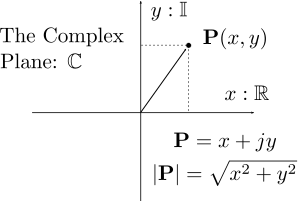
\includegraphics[scale=0.5]{images/lecture1_fig1.png} \\

				\large Is this a stable system? What does that mean?\\


				\btVFill
			\end{frame}

		
		% section I subsection II
		\subsection{\sectionIsubsectionIItitle}\label{sectionIsubsectionII}

			\begin{frame}
				\frametitle{\sectionIsubsectionIItitle}
				\bigskip

				\frametitle{Stability in Dynamic Systems}

				A dynamic system is stable if ...  \vspace{50mm}\\

				\btVFill
			\end{frame}

			\begin{frame}
				\frametitle{\sectionIsubsectionIItitle}
				\bigskip

				\btVFill
			\end{frame}


		% section I subsection III
		\subsection{\sectionIsubsectionIIItitle}\label{sectionIsubsectionIII}
			\begin{frame} 
				\frametitle{\sectionIsubsectionIIItitle}
				\bigskip

				\frametitle{Step Input Function}

				\Large Consider the model subject to a Step Input, $f(t)$. \vspace{3mm}\\
				\begin{multicols}{2}
				\includegraphics[scale=.15]{images/ferrari.jpg}  

				\scalebox{1.25}{$m\dot{v} +cv=f(t)$} 

				\[f(t) = \begin{cases} 
				      0 & t < 0 \\
				      F & t\geq 0 \\
				   \end{cases}
				\]

				\end{multicols}


				\btVFill
			\end{frame}	

			\begin{frame} 
				\frametitle{\sectionIsubsectionIIItitle}
				\bigskip

				\frametitle{Solution with Laplace Transforms Method - Step 1}

				\large The method of Laplace Transforms is shown. \vspace{5mm} \\

					\scalebox{1.15}{$\Lagr{\{m\dot{v} +cv}=F\}$ $ \implies$  $m [sV(s) -v(0) ] +cV(s)=\frac{F}{c}$}  \vspace{0mm} \\

					\scalebox{1.15}{$(ms+c)V(s)=\frac{F}{s}+mv(0)$}  \vspace{5mm} \\

				\large Solve for $V(s)$. \vspace{2mm} \\
					\scalebox{1.15}{$V(s)=\frac{F}{s(ms+c)}+\frac{mv(0)}{ms+c}$} 

			
				\btVFill
			\end{frame}	


			\begin{frame} 
				\frametitle{\sectionIsubsectionIIItitle}
				\bigskip
				\frametitle{Solution with Laplace Transforms Method - Step 2}

				Expand $V(s) $as a partial fraction. \vspace{2mm} \\
					\scalebox{1.15}{$V(s)=\frac{F}{s(ms+c)}+\frac{mv(0)}{ms+c}\implies \frac{F}{s(ms+c)}=\frac{a}{s} +\frac{b}{ms+c}$} \vspace{5mm} \\
				\large 'Cover up' to find the coefficients. \vspace{2mm} \\

					\scalebox{1.15}{$a=\frac{F}{m\times0+c} $ \hspace{5mm} and \hspace{5mm} $b=\frac{F}{\frac{-c}{m}}=\frac{-Fm}{c}$}  \vspace{2mm} \\

				\large This leads to a form that can be inverted with the table. \vspace{5mm} \\

				\scalebox{1.15}{$V(s)=\frac{F}{c}\{ \frac{1}{s}-\frac{1}{s+\frac{c}{m}}\}+\frac{v(0)}{s+\frac{c}{m}}$} 
			
				\btVFill
			\end{frame}	


			\begin{frame} 
				\frametitle{\sectionIsubsectionIIItitle}
				\bigskip

				\frametitle{Solution with Laplace Transforms Method - Step 3}

				Can you find these terms in the Table of Laplace Transforms? \vspace{5mm}\\
				\scalebox{1.15}{$V(s)=\frac{F}{c}\{ \frac{1}{s}-\frac{1}{s+\frac{c}{m}}\}+\frac{v(0)}{s+\frac{c}{m}}$}  \vspace{5mm} \\

				The inverse Laplace transform of $V(s)$ gives the time response. \vspace{5mm}\\

				\scalebox{1.15}{$v(t)=\frac{F}{C}\{1-e^{-\frac{t}{\tau}} \} + v(0)e^{-\frac{t}{\tau}} = \{v(0)-\frac{F}{c}\}e^{-\frac{t}{\tau}} + \frac{F}{c}$  }
					

			
				\btVFill
			\end{frame}	


			\begin{frame} 
				\frametitle{\sectionIsubsectionIIItitle}
				\bigskip

			
				\btVFill
			\end{frame}	


			\begin{frame} 
				\frametitle{\sectionIsubsectionIIItitle}
				\bigskip

			
				\btVFill
			\end{frame}	

		% section I subsection IV
		\subsection{\sectionIsubsectionIVtitle}\label{sectionIsubsectionIV}

			\begin{frame}
				\frametitle{\sectionIsubsectionIVtitle}
				\bigskip

				\frametitle{Sketch Response Equation}

				\large Sketch the System Response in the time Domain.  \vspace{3mm}\\

				\scalebox{1.25}{$v(t)=\{v(0)-\frac{F}{c}\}e^{-\frac{t}{\tau}} + \frac{F}{c}$ }  \vspace{3mm}\\

				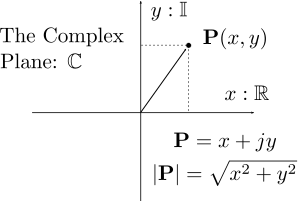
\includegraphics[scale=0.5]{images/lecture1_fig1.png} \\

				\large Is this a stable system?\\

				
		
				\btVFill
			\end{frame}	

			\begin{frame}
				\frametitle{\sectionIsubsectionIVtitle}
				\bigskip

				\frametitle{Components of the Response}

				\large In these forms we can see the different components of the response.\vspace{3mm}\\

				\scalebox{1.15}{$v(t)=\frac{F}{C}\{1-e^{-\frac{t}{\tau}} \} + v(0)e^{-\frac{t}{\tau}} = \{v(0)-\frac{F}{c}\}e^{-\frac{t}{\tau}} + \frac{F}{c}$  } \vspace{3mm}\\


				\large
				\begin{itemize}

				\item Forced Response\\

				\item Free Response\\

				\item Transient Response\\

				\item Steady-State Response

				\end{itemize}

			
				\btVFill
			\end{frame}	

			\begin{frame}
				\frametitle{\sectionIsubsectionIVtitle}
				\bigskip
				\frametitle{References}

				\begin{itemize}
					\item System Dynamics, Palm III, Third Edition - Section 8.1 - Response of First Order Systems - pg. 475
				\end{itemize}

			

				\btVFill
			\end{frame}

	
	% Section II
	\section{\sectionIItitle}\label{sectionII}

		% section II Outline
		\begin{frame}
			\large \textbf{Topic 2 - \sectionIItitle} \vspace{3mm}\\

			\begin{itemize}
				\item \hyperlink{sectionIIsubsectionI}{\sectionIIsubsectionItitle} \vspc %  section II subsection I
				\item \hyperlink{sectionIIsubsectionII}{\sectionIIsubsectionIItitle} \vspc % section II subsection II
				\item \hyperlink{sectionIIsubsectionIII}{\sectionIIsubsectionIIItitle} \vspc % section II subsection III
				\item \hyperlink{sectionIIsubsectionIV}{\sectionIIsubsectionIVtitle} \vspc % section II subsection IV
			\end{itemize}

		\end{frame}

		% section II subsection I
		\subsection{\sectionIIsubsectionItitle}\label{sectionIIsubsectionI}

			\begin{frame}[label=sectionIIsubsectionI]
				\frametitle{\sectionIIsubsectionItitle}
				\bigskip

				\frametitle{Mass Spring Model}

				\large Consider the mass-spring system without damping.\vspc

				\includegraphics[scale=.5]{images/mass_spring_01.png} \vspc

				\large The EOM is:\vspc

					\scalebox{1.0}{$m\ddot{x} +kx=0$\hspc with} \vspc
					\scalebox{1.0}{$ x(t=0)=x_0$, \hspc and\hspc$v(t=0)=v_0$}\vspc

								
				\btVFill
			\end{frame}

			\begin{frame}[label=sectionIIsubsectionI]
				\frametitle{\sectionIIsubsectionItitle}
				\bigskip

				\frametitle{Solution with Laplace Transforms Method}

				\large Solve for $x(t)$ with a method of your choice. \vspace{40mm}\\


				\scalebox{1.0}{$x(t)=\frac{v_0}{\omega_n}sin(\omega_nt)+x_0cos(w_nt) $\hspc with\hspc $\omega_n=\sqrt{\frac{k}{m}}$} \vspc


				\btVFill
			\end{frame}

			\begin{frame}[label=sectionIIsubsectionI]
				\frametitle{\sectionIIsubsectionItitle}
				\bigskip

				\frametitle{Phase Shift}

				\large The solution is commonly written as a single oscillating term with a {\bf phase shift} $\phi$.\vspc

					\scalebox{1.0}{$x(t)=\frac{v_0}{\omega_n}sin(\omega_nt)+x_0cos(w_nt) $\hspc with\hspc $\omega_n=\sqrt{\frac{k}{m}}$} \vspc

				\large Is equivalent to: \vspc

					\scalebox{1.0}{$x(t)=Acos(\omega_nt-\phi)$\hspc$A=\sqrt{x_0^2+[\frac{v_0}{\omega_n}]^2}$\hspc$\phi=tan^{-1}(\frac{v_0}{x_0\omega_n})$} \vspc

				\large Sine could be used instead.\vspc

				\scalebox{1.0}{$x(t)=Asin(\omega_nt+\phi)$\hspc$A=\sqrt{x_0^2+[\frac{v_0}{\omega_n}]^2}$\hspc$\phi=tan^{-1}(\frac{x(0)\omega_n}{v_0})$} \\

				
				\btVFill
			\end{frame}

			\begin{frame}[label=sectionIIsubsectionI]
				\frametitle{\sectionIIsubsectionItitle}
				\bigskip

				\frametitle{Sketch of Free Response}

				\large Sketch the {\bf free} response in the time domain.  \vspc

				\scalebox{1.0}{$x(t)=\frac{v_0}{\omega_n}sin(\omega_nt)+x_0cos(w_nt) $ }  \vspc
				\scalebox{1.0}{$=Acos(\omega_nt-\phi)$\hspc$with$\hspc$\phi=tan^{-1}(\frac{v_0}{x_0\omega_n})$}  \vspc

				\includegraphics[scale=0.5]{images/lecture2_fig2.png} \\

				\large Is this a stable system? What does the phase shift $\phi$ represent? \\

				
				\btVFill
			\end{frame}

			\begin{frame}[label=sectionIIsubsectionI]
				\frametitle{\sectionIIsubsectionItitle}
				\bigskip

				\frametitle{Second Order System with Damping}

				\large Now, consider the mass-spring system with damping present.\vspc

					\includegraphics[scale=.4]{images/mass_spring_02.png} \hspc \includegraphics[scale=.20]{images/beam_bending_01.png} 

				\large The EOM is:\vspc

					\scalebox{1.0}{$m\ddot{x} +c\dot{x}+kx=0$\hspc with} \vspc
					\scalebox{1.0}{$ x(t=0)=x_0$, \hspc and\hspc$v(t=0)=v_0$}\vspc

			
				\btVFill
			\end{frame}

			\begin{frame}[label=sectionIIsubsectionI]
				\frametitle{\sectionIIsubsectionItitle}
				\bigskip


				\frametitle{Solution with Trial Solution Method}

				The trial solution method is used to derive the response equation in terms of the system variables and parameters. \vspc

				%\large The affects of damping can be seen in the reponse equations.  \vspc

					\scalebox{1.0}{$m\ddot{x} +c\dot{x}+kx=0$ $ \implies$  $(mr^2+cr+k)Ae^{rt}=0$} \vspc

				\large You can see the {\it characteristic equation} becomes: \vspc
					\scalebox{1.0}{$(mr^2+cr+k)=0$}   \vspc

				\large Solve for the roots. In system dynamics they are called $s_{1,2}$  \vspc

					\scalebox{1.0}{$r_{1,2}=s_{1,2}=\frac{-c\pm\sqrt{c^2-4mk}}{2m}=-\frac{c}{2m}\pm\sqrt{(\frac{c}{2m})^2-\frac{k}{m}}$}   \vspc

			
				\btVFill
			\end{frame}


			\begin{frame}[label=sectionIIsubsectionI]
				\frametitle{\sectionIIsubsectionItitle}
				\bigskip

				\frametitle{The Roots of the System}

				\large The roots of the system determine the behavior.  \vspc

				\scalebox{1.0}{$s_{1,2}=\frac{-c\pm\sqrt{c^2-4mk}}{2m}$}\vspc

				The {\bf discriminant} $c^2-4mk$ drives the {\it case} in the trial solution method. \vspc

				\begin{itemize}
				\item IF \underline{\hspace{20mm}} $\implies$Case 1: Distinct and Real \vspace{1mm}\\
				\item IF \underline{\hspace{20mm}} $\implies$Case 2: Repeated and Real \vspace{1mm}\\
				\item IF \underline{\hspace{20mm}} $\implies$Case 3: Complex Conjugate Pair \vspc
				\end{itemize}

			
				\btVFill
			\end{frame}


			\begin{frame}[label=sectionIIsubsectionI]
				\frametitle{\sectionIIsubsectionItitle}
				\bigskip

				\frametitle{Damping Cases and the Critical Damping Value}

				\large In a system with known mass and spring constant, the damping value determines the behavior. The damping value that causes the {\it discriminant} to equal zero (case 2) is the {\bf critical damping value}.  \vspc

				\scalebox{1}{$c^2-4mk = 0 \implies c=\sqrt{4mk}=2\sqrt{mk}$} \vspcc

				\scalebox{1}{$c_{critical}=2\sqrt{mk}$} \vspc


			
				\btVFill
			\end{frame}



			\begin{frame}[label=sectionIIsubsectionI]
				\frametitle{\sectionIIsubsectionItitle}
				\bigskip

				\frametitle{The Damping Ratio}

				\large The damping ratio $\zeta$ is the ratio of damping c to the critical damping value $c_{critical}$. \vspace{2mm}\\

				\scalebox{1.0}{$\zeta=\frac{c}{c_{critical}}=\frac{c}{2\sqrt{mk}}$} \vspace{2mm}\\

				\large Re-write the roots with this new quantity. \vspace{2mm}\\

				\scalebox{1.0}{$s_{1,2}=-\zeta\omega_n\pm\omega_n\sqrt{\zeta^2-1}=-\zeta\omega_n\pm j\omega_n\sqrt{1-\zeta^2}$}  \vspace{2mm}\\

				\large We define a new quantity, {\bf damped natural frequency}.  \vspace{2mm}\\
					
				\scalebox{1.0}{$\omega_d=\omega_n\sqrt{1-\zeta^2}$}  \vspace{2mm}\\

				\large Now re-write the roots again in terms of $\zeta$ and $\omega_d$.  \vspace{2mm}\\

				\scalebox{1.0}{$s_{1,2}=\zeta\omega_n\pm j\omega_d$}  \vspace{2mm}\\
							
				\btVFill
			\end{frame}


			\begin{frame}[label=sectionIIsubsectionI]
				\frametitle{\sectionIIsubsectionItitle}
				\bigskip

				\large The behavior of the system depends on the damping ratio.  \vspcc


				\renewcommand{\arraystretch}{2}
				\begin{tabular}{|c|c|c|c|}
				Case 1&\scalebox{1.0}{$c>2\sqrt{mk}$ }&{\bf Overdamped}&\scalebox{1}{$\zeta>1$} \\
				Case 2&\scalebox{1.0}{$c=2\sqrt{mk}=c_{critical}$ }&{\bf Critically Damped}&\scalebox{1}{$\zeta=1$}\\
				Case 3&\scalebox{1.0}{$c<2\sqrt{mk}$ }&{\bf Underdamped}&\scalebox{1}{$\zeta<1$} \\
				\end{tabular}

			
				\btVFill
			\end{frame}



		% section II subsection II
		\subsection{\sectionIIsubsectionIItitle}\label{sectionIIsubsectionII}

			\begin{frame}

				\frametitle{\sectionIIsubsectionIItitle}
				\bigskip

				The roots are real and distinct and the system {\it does not} oscillate. \vspc

				\large \underline{Overdamped}\hspc $c>2\sqrt{mk} \hspc \implies\hspc \zeta>1$ \hspc \vspcc

				\scalebox{1}{$s_{1,2}=-\zeta\pm\omega_n\sqrt{\zeta^2-1}$}\vspc

				\scalebox{1}{$x(t)=C_1e^{(-\zeta\omega_n+\omega_n\sqrt{\zeta^2-1}\hspace{1mm})t}+C_2e^{(-\zeta\omega_n-\omega_n\sqrt{\zeta^2-1}\hspace{1mm})t}$}\vspc

				\scalebox{1}{$x(t)=e^{-\zeta\omega_n}\{C_1e^{\omega_n\sqrt{\zeta^2-1}t}+C_2e^{\omega_n\sqrt{\zeta^2-1}t}\}$}\vspc
				\scalebox{1}{$C_1=\frac{-v_0+(-\zeta+\sqrt{\zeta^2-1})\omega_nx_0}{2\omega_n\sqrt{\zeta^2-1}}$}\hspc
				\scalebox{1}{$C_2=\frac{-v_0+(\zeta+\sqrt{\zeta^2-1})\omega_nx_0}{2\omega_n\sqrt{\zeta^2-1}}$} \vspc


				\btVFill 
			\end{frame}

			



		% section II subsection III
		\subsection{\sectionIIsubsectionIIItitle}\label{sectionIIsubsectionIII}

			\begin{frame}
				\frametitle{\sectionIIsubsectionIIItitle}
				\bigskip
				\frametitle{The Critically Damped Case}

				The roots are real and repeated and the system {\it does not} oscillate. \vspcc

				\large \underline{Critically Damped}\hspc $c=2\sqrt{mk} \hspc \implies\hspc \zeta=1$ \hspc \vspcc

				\scalebox{1}{$s_{1,2}=\frac{-c}{2m}=\zeta\omega_n=-\omega_n$}\vspc

				\scalebox{1}{$x(t)=C_1e^{-\omega_nt}+C_2te^{-\omega_nt}$}\vspc

				\scalebox{1}{$\dot{x}=-\omega_nC_1e^{-\omega_nt}+C_2t(-\omega_ne^{-\omega_nt})+e^{-\omega_nt}(C_2)$} \vspc

				\scalebox{1}{$x(t=0)=x_0\implies C_1=x_0$}\vspc

				\scalebox{1}{$v(t=0)=v_0\Rightarrow v_0=-\omega_nC_1+0+(1)C_2 \implies C_2=v_0+\omega_nx_0$}\vspc


				\btVFill 
			\end{frame}	



			
		% section II subsection IV
		\subsection{\sectionIIsubsectionIVtitle}\label{sectionIIsubsectionIV}

			\begin{frame}[containsverbatim]
				\frametitle{\sectionIIsubsectionIVtitle}
				\bigskip

				\frametitle{The Underdamped Case}

				Take the derivative and solve for the second unknown. \vspc

				\scalebox{1}{$x(t)=e^{-\zeta\omega_nt}\{Acos(\omega_dt)+Bsin(\omega_dt)\}$}\vspc

				\scalebox{1}{$\dot{x}(t)=e^{-\zeta\omega_nt}(-\omega_dAsin(\omega_dt))+Acos(\omega_dt)(-\zeta\omega_ne^{-\zeta\omega_nt})$}\vspc

				\scalebox{1}{$+e^{-\zeta\omega_nt}(\omega_dBcos(\omega_dt))+Bsin(\omega_dt)e^{-\zeta\omega_nt}$}\vspc

				\scalebox{1}{$\dot{x}(t=0)=A(1)(-\zeta\omega_n(1))+(1)\omega_dB(1)\implies B=\frac{v_0+\zeta\omega_nx_0}{\omega_d}$}\vspc

				Finally we get to the reponse equation. \vspc

				\scalebox{1}{$x(t)=e^{-\zeta\omega_nt}\{x_0cos(\omega_dt)+\frac{v_0+\zeta\omega_nx_0}{\omega_d}sin(\omega_dt)\}$}


				\btVFill 
			\end{frame}	

			\begin{frame}
				\frametitle{\sectionIIsubsectionIVtitle}
				\bigskip

				\frametitle{Response of the Three Different Cases}

				\large Each of the three cases behaves in a {\it characteristic} way.\vspcc
				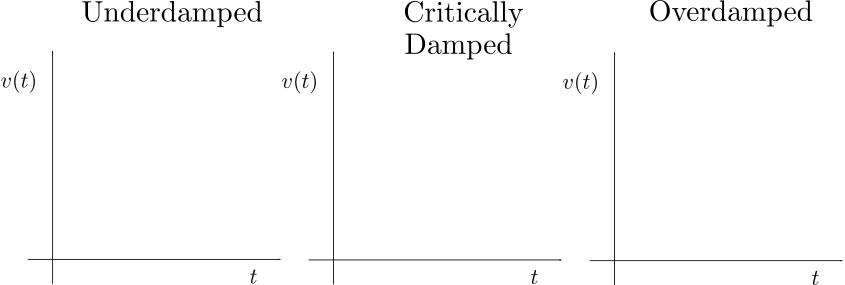
\includegraphics[scale=0.5]{images/lecture2_fig3.png} 

				\btVFill 
			\end{frame}		
				

			\begin{frame}
				\frametitle{\sectionIIsubsectionIVtitle}
				\bigskip

				\frametitle{Affects of Damping Ratio and Damped Natural Frequency}

				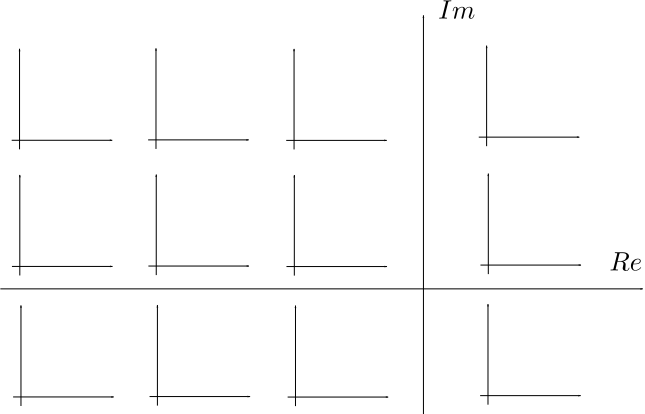
\includegraphics[scale=0.60]{images/lecture2_fig4.png} 

				\btVFill 
			\end{frame}	
		
	% Section III
	\section{\sectionIIItitle}\label{sectionIII}

		% section III Outline
		\begin{frame}
			\large \textbf{Topic 3 - \sectionIIItitle} \vspace{3mm}\\

			\begin{itemize}
				\item \hyperlink{sectionIIIsubsectionI}{\sectionIIIsubsectionItitle} \vspc %  section III subsection I
				\item \hyperlink{sectionIIIsubsectionII}{\sectionIIIsubsectionIItitle} \vspc % section III subsection II
				\item \hyperlink{sectionIIIsubsectionIII}{\sectionIIIsubsectionIIItitle} \vspc % section III subsection III
				\item \hyperlink{sectionIIIsubsectionIV}{\sectionIIIsubsectionIVtitle} \vspc % section III subsection IV
			\end{itemize}

		\end{frame}

		% section III subsection I
		\subsection{\sectionIIIsubsectionItitle}\label{sectionIIIsubsectionI}

			\begin{frame}
				\frametitle{\sectionIIIsubsectionItitle}
				\bigskip

				\frametitle{Affect of Root Location on Response}
 	
				The {\it location} of the root in the {\it complex plane} shows the affects of the roots on the system behviour.\vspc
				\includegraphics[scale=0.4]{images/lecture3_fig5.png}

				\btVFill
			\end{frame}

			\begin{frame}
				\frametitle{\sectionIIIsubsectionItitle}
				\bigskip

				


				\btVFill
			\end{frame}

		% section III subsection II
		\subsection{\sectionIIIsubsectionIItitle}\label{sectionIIIsubsectionII}	

			\begin{frame}
				\frametitle{\sectionIIIsubsectionIItitle}
				\bigskip

				\frametitle{Along a Vertical Line}
 	
				As the root moves along a vertical line...\vspc
				\includegraphics[scale=0.5]{images/lecture3_fig2.png}


				\btVFill
			\end{frame}

			\begin{frame}
				\frametitle{\sectionIIIsubsectionIItitle}
				\bigskip


				\btVFill
			\end{frame}

		% section III subsection III
		\subsection{\sectionIIIsubsectionIIItitle}\label{sectionIIIsubsectionIII}

			\begin{frame}
				\frametitle{\sectionIIIsubsectionIIItitle}
				\bigskip

				\frametitle{Along a Horizontal Line}
 	
				As the root moves along a horizontal line...\vspc
				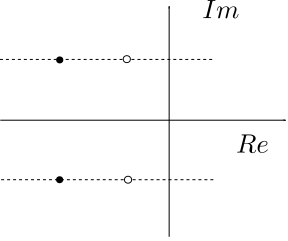
\includegraphics[scale=0.5]{images/lecture3_fig3.png}
				
	
				\btVFill
			\end{frame}

			\begin{frame}
				\frametitle{\sectionIIIsubsectionIIItitle}
				\bigskip


				\btVFill
			\end{frame}

			\begin{frame}
				\frametitle{\sectionIIIsubsectionIIItitle}
				\bigskip

				\btVFill
			\end{frame}

		% section III subsection IV
		\subsection{\sectionIIIsubsectionIVtitle}\label{sectionIIIsubsectionIV}	

			\begin{frame}[containsverbatim]
				\frametitle{\sectionIIIsubsectionIVtitle}
				\bigskip

				\frametitle{Along a Diagonal Line}
 	
				As the root moves along a diagonal line...\vspc
				\includegraphics[scale=0.5]{images/lecture3_fig4.png}

				What about the angle of this line?

				\btVFill 
			\end{frame}



	% Section IV
	\section{\sectionIVtitle}\label{sectionIV}

		% section IV Outline
		\begin{frame}
			\large \textbf{Topic 3 - \sectionIVtitle} \vspace{3mm}\\

			\begin{itemize}
				\item \hyperlink{sectionIVsubsectionI}{\sectionIVsubsectionItitle} \vspc %  section III subsection I
				\item \hyperlink{sectionIVsubsectionII}{\sectionIVsubsectionIItitle} \vspc % section III subsection II
				\item \hyperlink{sectionIVsubsectionIII}{\sectionIVsubsectionIIItitle} \vspc % section III subsection III
				\item \hyperlink{sectionIVsubsectionIV}{\sectionIVsubsectionIVtitle} \vspc % section III subsection IV

			\end{itemize}

		\end{frame}

		% section IV subsection I
		\subsection{\sectionIVsubsectionItitle}\label{sectionIVsubsectionI}

			\begin{frame}
				\frametitle{\sectionIVsubsectionItitle}
				\bigskip

				\frametitle{The Mass Spring Damper}

				\large Now, consider the mass-spring system with damping present subject to {\bf step} input. This models instantly turning on the input force $f(t)$.\vspc

				\begin{multicols}{2}

					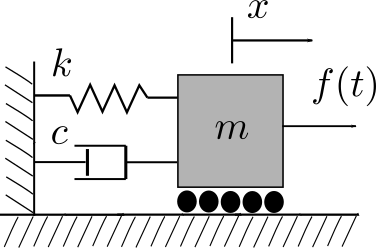
\includegraphics[scale=.4]{images/mass_spring_04.png} \hspc  

					\underline{Heavyside's Step Function}\vspc
					\[f(t) = \begin{cases} 
					      0 & t < 0 \\
					      F & t\geq 0 \\
					   \end{cases}
					\]

				\end{multicols}

				\large The EOM is:

					\[ m\ddot{x} +c\dot{x}+kx=f(t) \hspcc with \hspc x(t=0)=x_0 \hspcc and \hspcc v(t=0)=v_0 \] 

				\btVFill
			\end{frame}

			\begin{frame}
				\frametitle{\sectionIVsubsectionItitle}
				\bigskip

				\frametitle{Unit Step Response}
				The {\bf unit step response} is a special case of the {\it forced response} in which $f(t)$ is the step function of unit magnitude (F=1). \vspcc
				\renewcommand{\arraystretch}{2}
				\begin{tabular}{|c|c|}
				Overdamped & $ x(t)=\frac{1}{k}(\frac{r_2}{r_1-r_2}e^{-r_1t}-\frac{r_1}{r_1-r_2}e^{-r_2t}+1 $ \\
				& $r_{1,2}=-s_{1,2}$ \\
				Critically Damped & $ x(t)=\frac{1}{K}[(-1-\omega_nt)e^{-\omega_nt}+1] $ \\
				Underdamped & $ x(t)=\frac{1}{k}\left[\frac{1}{\sqrt{1-\zeta^2}}e^{-\zeta\omega_nt}sin(\omega_dt+\phi+1\right] $ \\
				& $ \phi=tan^{-1}\left(\frac{\sqrt{1-\zeta^2}}{\zeta}\right)+\pi $ \\
				\end{tabular}
			
				
				\btVFill
			\end{frame}

		% section IV subsection II
		\subsection{\sectionIVsubsectionIItitle}\label{sectionIVsubsectionII}	

			\begin{frame}
				\frametitle{\sectionIVsubsectionIItitle}
				\bigskip


				We are going to derive several quatities that describes the response of an underdamped system. \vspc

				\includegraphics[scale=0.7]{images/lecture3_fig1.png}

				\btVFill
			\end{frame}

			\begin{frame}
				\frametitle{\sectionIVsubsectionIItitle}
				\bigskip

				\frametitle{Rise Time}

				The {\bf rise time} is the time at which the response first equals the steady state value.\vspc

				%\includegraphics[scale=0.35]{lecture3_fig1.png}\vspc
				\[ x(t)=\frac{1}{k}\left[\frac{1}{\sqrt{1-\zeta^2}}e^{-\zeta\omega_nt}sin(\omega_dt+\phi)+1\right] \] 

				Set the {\it transient term} to zero and solve for $t$.\vspc
				\[ e^{-\zeta\omega_nt}sin(\omega_dt+\phi)=0 \implies sin(\omega_dt+\phi)=0\implies \omega_dt+\phi=2\pi \]
				\[ t_{rise}=t_r=\frac{2\pi-\phi}{\omega_d} \]


				\btVFill
			\end{frame}

			\begin{frame}
				\frametitle{\sectionIVsubsectionIItitle}
				\bigskip

				The {\bf peak time} is the time at which the response equals the maximum value. Find the derivative of the response equation and set it equal to zero. \vspc

				\[ \dot{x}(t)= \]
				\[ \left(\frac{1}{K}\frac{1}{\sqrt{1-\zeta^2}}\right)\left[ e^{-\zeta\omega_nt}(\omega_dcos(\omega_dt+\phi))+sin(\omega_dt+\phi)(-\zeta\omega_ne^{-\zeta\omega_nt})\right] \] 
				%\includegraphics[scale=0.7]{lecture3_fig1.png}
				\[ sin(\omega_d)t=0\implies \omega_dt=\pi \implies \hspc t_{peak}= t_p=\frac{\pi}{\omega_d} \] 


				\btVFill
			\end{frame}


			\begin{frame}
				\frametitle{\sectionIVsubsectionIItitle}
				\bigskip


				The {\bf settling time} is the time at which the response decays to a certain percentage of the steady state value.\vspc

				It can be esitmated as:\vspc
				\[ t_{settling}=t_s=-\frac{ln(tolerance)}{\zeta\omega_n} \] 
				\[ 2\%\implies tolerance=0.02 \]
				\[ 5\%\implies tolerance=0.05 \]
				%\includegraphics[scale=0.7]{lecture3_fig1.png}


				\btVFill
			\end{frame}

			\begin{frame}
				\frametitle{\sectionIVsubsectionIItitle}
				\bigskip


				The {\bf maximum overshoot} is the response beyond the steady state value. \vspc

				\[ M_p=x(t_p)-x_{ss}\implies M_p=\frac{1}{k}e^{\frac{-\pi\zeta}{\sqrt{1-\zeta^2}}} \]

				This is often expressed as a percentage. \vspc

				\[ M_\%=\frac{x(t_p)-x_{ss}}{x_{ss}}100=100e^{\frac{-\pi\zeta}{\sqrt{1-\zeta^2}} } \]

				%=100e^{-\frac{\pi\zeta}{\sqrt{1-\zeta^2}}}$}
				%\includegraphics[scale=0.7]{lecture3_fig1.png}


				\btVFill
			\end{frame}


		% section IV subsection III
		\subsection{\sectionIVsubsectionIIItitle}\label{sectionIVsubsectionIV}

			\begin{frame}
				\frametitle{\sectionIVsubsectionIIItitle}
				\bigskip

				\frametitle{Damping Ratio from Maximum Overshoot}

				The {\it damping ratio} can be determined from the maximum overshoot! \vspc

				\[ M_\%=100e^{\frac{-\pi\zeta}{\sqrt{1-\zeta^2}}} \]\vspc

				Solve for $\zeta$.\vspc

				\[ \zeta=\frac{R}{\sqrt{\pi^2+R^2}} \hspc with \hspc R=ln\left(\frac{100}{M\%}\right) \]


				\btVFill
			\end{frame}

			\begin{frame}
				\frametitle{\sectionIVsubsectionIIItitle}
				\bigskip

				\frametitle{Damping Ratio from Log Decrement}

				The logarithmic decrement is the natural log of the ratio of the amplitudes of any two successive peaks: 
				\[ \delta=\frac{1}{n}ln\frac{x(t)}{x(t+nT)} \]

				x(t) is the overshoot (amplitude - final value) at time t and x(t + nT) is the overshoot of the peak n periods away. \vspc

				The damping ratio is then found from the logarithmic decrement by: 

				\[ \zeta=\frac{1}{\sqrt{1+\left(\frac{2\pi}{\delta}\right)^2}} \]

				\btVFill
			\end{frame}

			\begin{frame}
				\frametitle{\sectionIVsubsectionIIItitle}
				\bigskip

				\frametitle{Damping Ratio from Log Decrement}

				What is the significance of all of this? \vspc
				Why do we care about all of these new parameters?

				\btVFill
			\end{frame}

		% section IV subsection IV
		\subsection{\sectionIVsubsectionIVtitle}\label{sectionIVsubsectionIV}	

			\begin{frame}
				\frametitle{\sectionIVsubsectionIVtitle}
				\bigskip
	

				\btVFill 
			\end{frame}

			\begin{frame}
				\frametitle{\sectionIVsubsectionIVtitle}
				\bigskip

			

		 		\btVFill 
			\end{frame}
			
			\begin{frame}
				\frametitle{\sectionIVsubsectionIVtitle}
				\bigskip
				
				
					
				\btVFill 
			\end{frame}

			\begin{frame}
				\frametitle{\sectionIVsubsectionIVtitle}
				\bigskip
			
				
				\btVFill 
			\end{frame}



\end{document}





